\documentclass[12pt,a4paper]{article}

\usepackage{geometry}
\geometry{margin=1.2in}

\usepackage{amsmath,amssymb}
\usepackage{booktabs}
\usepackage{hyperref}
\usepackage{microtype}
\usepackage{graphicx}
\usepackage{natbib}
\usepackage{caption}
\usepackage{pgfplots}
\pgfplotsset{compat=1.18}
\usepackage{pgfplotstable}

\title{Developer Lifecycles and Language Ecosystem Dynamics on GitHub:\\
A Large-Scale Analysis of a Follow Network}

\author{Flyxion}
\date{\today}

\begin{document}

\maketitle

\begin{abstract}
We present a large-scale empirical analysis of developer activity on GitHub using a dataset constructed from a follow network exceeding one million accounts. Unlike prior work focused on repositories, this study adopts a developer-centered perspective, tracking activity lifecycles at the level of individual users. Using metadata collected via the GitHub GraphQL API, we classify accounts as active or inactive based on recent commit activity and associate each developer with a primary programming language inferred from their most recently updated repository. Analysis of approximately $370{,}000$ accounts reveals a characteristic developer activity half-life of approximately ten years, strong variation in activity across programming language ecosystems, and evidence of generational turnover in software ecosystems. These findings provide a quantitative framework for understanding the temporal structure of developer participation in open source systems.
\end{abstract}

\section{Introduction}

The growth of open source software has transformed software development into a large-scale, globally distributed process. GitHub, as one of the central platforms for this activity, provides an unprecedented observational window into developer behavior, collaboration patterns, and the evolution of programming language ecosystems.

Most empirical studies of GitHub rely on repository-centric datasets such as GitHub Archive or BigQuery mirrors. While these datasets capture detailed event histories, they primarily describe \emph{artifacts} rather than \emph{actors}. As a result, they provide limited insight into the lifecycle of individual developers.

This paper adopts a complementary perspective by analyzing GitHub as a population of developers. Rather than tracking repositories, we track users: their entry into the system, their persistence over time, and their association with programming language ecosystems. The central questions we address concern what fraction of developers remain active over time, whether there is a characteristic lifetime of developer activity, how activity varies across programming language ecosystems, and what structural patterns emerge at scale. To answer these questions, we construct a large dataset derived from a GitHub follow network and analyze activity using survival-style methods and ecosystem-level aggregation.

\section{Related Work}

Empirical studies of GitHub have traditionally focused on repository dynamics, collaboration networks, and event streams \citep{kalliamvakou2014promises, gousios2014ghtorrent}. These studies have provided valuable insights into pull request workflows, project growth, and contribution patterns.

More recent work has explored developer behavior, including onboarding, retention, and collaboration structures \citep{zhou2016information, joblin2017classifying}. However, most analyses rely on indirect measures of activity derived from repository events rather than explicit modeling of developer lifecycles. Survival analysis has been applied in related contexts, such as developer retention in open source communities and user churn in online platforms \citep{vasilescu2015gender}, suggesting that participation in software ecosystems exhibits measurable temporal structure.

The present work differs from prior studies in two key respects. First, it uses a developer-centered dataset derived from a follow network rather than repository events. Second, it explicitly models activity as a function of account age, enabling estimation of developer lifetimes and ecosystem-specific retention.

\section{Dataset Construction}

\subsection{Sampling Strategy}

The dataset is constructed by crawling the follow graph of a GitHub user with an exceptionally large number of followed accounts, on the order of one million. This produces a population of developers that is not uniformly random but is instead biased toward socially visible or interconnected accounts. While this introduces sampling bias, it also yields a population enriched for active and engaged developers, making it particularly suitable for studying sustained participation.

\subsection{Data Collection}

Data is collected using the GitHub GraphQL API in batched queries. For each account, we retrieve the account creation timestamp $t_{\text{create}}$, the number of followers, the number of public repositories, the most recently pushed repository, the timestamp of the most recent push $t_{\text{push}}$, and the primary language of that repository. Accounts that cannot be resolved as users---such as organizations or deleted accounts---are excluded from analysis.

\subsection{Activity Classification}

We define a binary activity indicator:
\[
A =
\begin{cases}
1 & \text{if } t_{\text{push}} \geq t_{\text{now}} - \Delta \\
0 & \text{otherwise,}
\end{cases}
\]
where $\Delta = 365$ days. Thus, a developer is classified as \textbf{active} if they have pushed to a public repository within the past year, and \textbf{inactive} otherwise.

\subsection{Language Assignment}

Each developer is assigned a primary programming language based on the most recently updated repository. While this is a coarse proxy, it captures the developer's current ecosystem affiliation. Accounts with no identifiable primary language are assigned to a special category denoted \texttt{None}.

\subsection{Dataset Size}

At the time of analysis, the dataset contains $370{,}447$ total accounts, of which $215{,}442$ are classified as active and $155{,}005$ as inactive. This scale is sufficient to produce stable estimates of aggregate behavior and ecosystem-level structure.

\section{Methodology}

\subsection{Activity Ratio}

For each programming language $L$, we define the activity ratio:
\[
R(L) = \frac{N_{\text{active}}(L)}{N_{\text{active}}(L) + N_{\text{inactive}}(L)}.
\]
This metric estimates the probability that a developer associated with language $L$ is currently active.

\subsection{Account Age and Survival Function}

We define account age as $\tau = t_{\text{now}} - t_{\text{create}}$. Accounts are grouped into integer year bins, and the fraction of active accounts is computed for each bin. We approximate a survival function:
\[
S(\tau) = P(\text{active} \mid \text{age} = \tau),
\]
which represents the probability that a developer remains active at age $\tau$. The point at which $S(\tau) \approx 0.5$ provides an estimate of the \emph{activity half-life}.

\subsection{Observed Lifetime}

For each account with valid timestamps, we define an observed lifetime:
\[
\ell = t_{\text{push}} - t_{\text{create}}.
\]
This is a lower-bound estimate of the true lifetime, as currently active users are right-censored. Median lifetimes are computed for each language ecosystem.

\section{Results}

\subsection{Global Activity Rate}

Across the dataset of $370{,}447$ accounts, approximately $58.2\%$ are classified as active under the one-year activity threshold. This is notably higher than estimates derived from repository-centric datasets, reflecting the sampling bias inherent in follow networks toward socially connected or visible developers.

\subsection{Language Ecosystem Activity}

Table~\ref{tab:language-activity} presents activity ratios for the most common programming languages in the dataset. The results exhibit a clear stratification of ecosystems. Modern languages such as Rust and TypeScript show the highest activity ratios, indicating strong ongoing engagement and relatively few legacy inactive accounts. In contrast, older ecosystems such as Ruby and Java display substantially lower activity ratios, reflecting the accumulation of inactive users over time.

\begin{table}[h]
\centering
\begin{tabular}{lrrr}
\toprule
Language & Active & Inactive & Activity Ratio \\
\midrule
Rust        & 4{,}805  &    976   & 0.831 \\
TypeScript  & 27{,}307 &  5{,}974 & 0.820 \\
Lua         & 1{,}555  &    390   & 0.799 \\
Dart        & 1{,}372  &    556   & 0.712 \\
Go          & 5{,}676  &  2{,}365 & 0.706 \\
Shell       & 5{,}352  &  2{,}323 & 0.697 \\
Python      & 40{,}229 & 17{,}920 & 0.692 \\
Kotlin      & 1{,}831  &    848   & 0.683 \\
HTML        & 16{,}455 &  8{,}400 & 0.662 \\
Swift       & 1{,}477  &    809   & 0.646 \\
JavaScript  & 20{,}087 & 13{,}404 & 0.600 \\
C++         & 6{,}821  &  4{,}736 & 0.590 \\
C\#         & 3{,}612  &  2{,}793 & 0.564 \\
PHP         & 2{,}749  &  2{,}303 & 0.544 \\
Java        & 6{,}297  &  6{,}246 & 0.502 \\
Ruby        & 1{,}582  &  2{,}098 & 0.430 \\
\bottomrule
\end{tabular}
\caption{Activity ratios for major programming languages, ordered by activity ratio.}
\label{tab:language-activity}
\end{table}

\subsection{The Null Language Population}

A significant fraction of accounts are associated with no identifiable primary language, with $N_{\text{None}} = 95{,}447$ and $R_{\text{None}} = 0.356$. This group dominates the inactive population, accounting for nearly $40\%$ of inactive accounts. It likely corresponds to users with no public repositories, archived projects, or non-code usage of the platform. The markedly lower activity ratio of this group suggests that repository presence is a strong predictor of continued participation.

\subsection{Distribution of Languages Among Active and Inactive Accounts}

The distribution of languages differs significantly between active and inactive populations. Among active accounts, the leading languages are Python at $18.67\%$, followed by the \texttt{None} category at $15.75\%$, TypeScript at $12.67\%$, JavaScript at $9.32\%$, and HTML at $7.64\%$. Among inactive accounts, the distribution is dominated by \texttt{None} at $39.68\%$, with Python at $11.56\%$, JavaScript at $8.65\%$, HTML at $5.42\%$, and Java at $4.03\%$. The contrast highlights the central role of the \texttt{None} category in accounting for inactivity and suggests that language ecosystems with active repository maintenance strongly correlate with continued engagement. Figure~\ref{fig:composition} illustrates this contrast directly.

\begin{figure}[h]
\centering
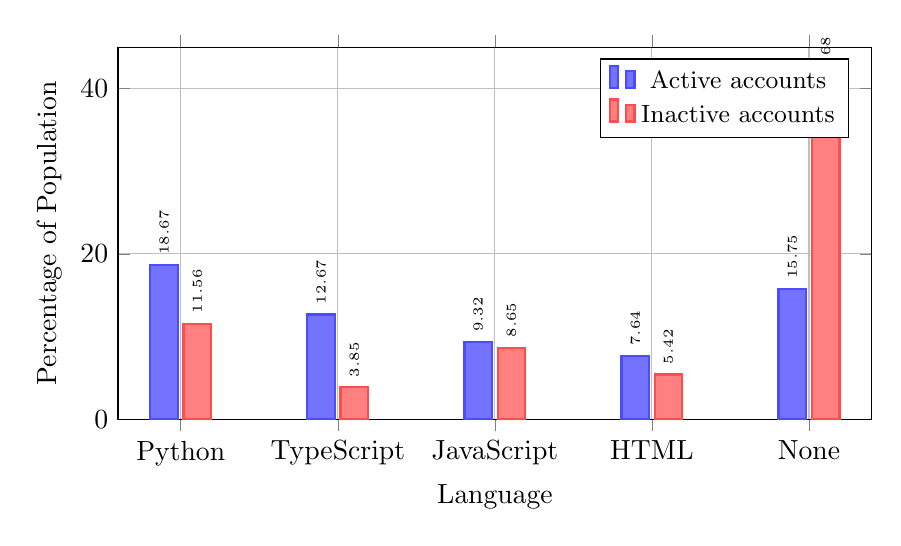
\begin{tikzpicture}
\begin{axis}[
    width=0.92\textwidth,
    height=0.52\textwidth,
    ybar,
    bar width=10pt,
    xlabel={Language},
    ylabel={Percentage of Population},
    symbolic x coords={Python,TypeScript,JavaScript,HTML,None},
    xtick=data,
    legend pos=north east,
    legend style={font=\small},
    grid=major,
    ymin=0, ymax=45,
    nodes near coords,
    nodes near coords style={font=\tiny, rotate=90, anchor=west},
    every axis plot/.append style={thick},
]
\addplot[fill=blue!55, draw=blue!70] coordinates {
    (Python,18.67)
    (TypeScript,12.67)
    (JavaScript,9.32)
    (HTML,7.64)
    (None,15.75)
};
\addplot[fill=red!50, draw=red!70] coordinates {
    (Python,11.56)
    (TypeScript,3.85)
    (JavaScript,8.65)
    (HTML,5.42)
    (None,39.68)
};
\legend{Active accounts, Inactive accounts}
\end{axis}
\end{tikzpicture}
\caption{Language distribution among active and inactive accounts. The \texttt{None} category is disproportionately concentrated among inactive accounts, while TypeScript shows a strong skew toward active participants.}
\label{fig:composition}
\end{figure}

\subsection{Developer Survival Curve}

Figure~\ref{fig:survival} presents the estimated survival function of developer activity as a function of account age, and Table~\ref{tab:survival} provides the underlying numerical values. The survival curve exhibits a gradual decline over the first decade, followed by stabilization and an eventual increase for older accounts. The point at which $S(\tau) \approx 0.5$ occurs near $\tau \approx 10$ years, suggesting a characteristic developer activity half-life of approximately ten years. The increase in activity fraction for older accounts is attributable to survivorship bias: early adopters who remain active are disproportionately persistent developers.

\begin{figure}[h]
\centering
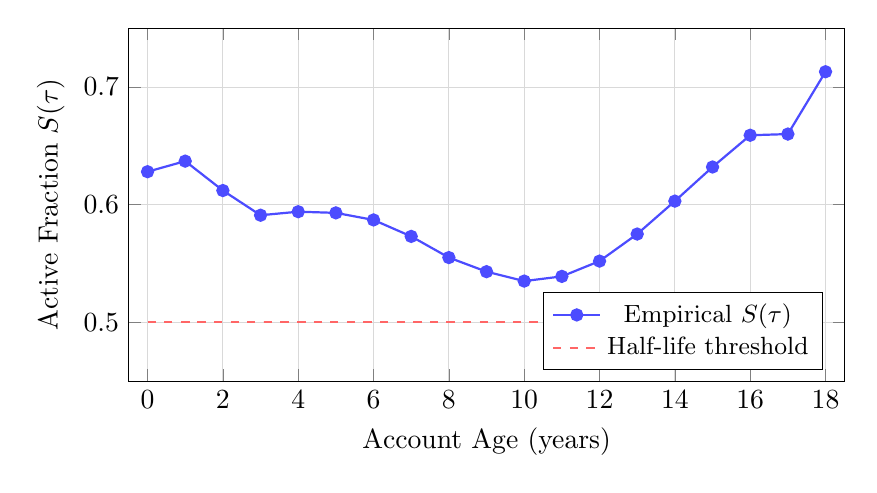
\begin{tikzpicture}
\begin{axis}[
    width=0.88\textwidth,
    height=0.50\textwidth,
    xlabel={Account Age (years)},
    ylabel={Active Fraction $S(\tau)$},
    ymin=0.45, ymax=0.75,
    xmin=-0.5, xmax=18.5,
    grid=both,
    grid style={line width=0.3pt, draw=gray!30},
    every axis plot/.append style={thick},
    legend pos=south east,
    legend style={font=\small},
]
\addplot[
    color=blue!70,
    mark=*,
    mark size=2pt,
] coordinates {
(0,0.628)(1,0.637)(2,0.612)(3,0.591)(4,0.594)(5,0.593)
(6,0.587)(7,0.573)(8,0.555)(9,0.543)(10,0.535)
(11,0.539)(12,0.552)(13,0.575)(14,0.603)(15,0.632)
(16,0.659)(17,0.660)(18,0.713)
};
\addlegendentry{Empirical $S(\tau)$}
\addplot[
    dashed,
    color=red!60,
    domain=0:18,
    samples=100,
] {0.5};
\addlegendentry{Half-life threshold}
\end{axis}
\end{tikzpicture}
\caption{Empirical survival function $S(\tau)$: fraction of accounts remaining active as a function of account age in years. The dashed line marks the $S(\tau) = 0.5$ threshold, intersected near $\tau \approx 10$ years. The upturn for accounts older than twelve years reflects survivorship bias among persistent early adopters.}
\label{fig:survival}
\end{figure}

\begin{table}[h]
\centering
\begin{tabular}{cc}
\toprule
Age (years) & Active Fraction $S(\tau)$ \\
\midrule
0  & 0.628 \\
1  & 0.637 \\
2  & 0.612 \\
3  & 0.591 \\
4  & 0.594 \\
5  & 0.593 \\
6  & 0.587 \\
7  & 0.573 \\
8  & 0.555 \\
9  & 0.543 \\
10 & 0.535 \\
11 & 0.539 \\
12 & 0.552 \\
13 & 0.575 \\
14 & 0.603 \\
15 & 0.632 \\
16 & 0.659 \\
17 & 0.660 \\
18 & 0.713 \\
\bottomrule
\end{tabular}
\caption{Estimated survival function $S(\tau)$ of developer activity by account age.}
\label{tab:survival}
\end{table}

\subsection{Language Activity Ratios}

Figure~\ref{fig:ratios} displays the activity ratios for the twenty-five largest language populations in the dataset. The ordering reveals a clear temporal gradient: recently established ecosystems cluster toward the top, while mature or legacy ecosystems occupy the lower range.

\begin{figure}[h]
\centering
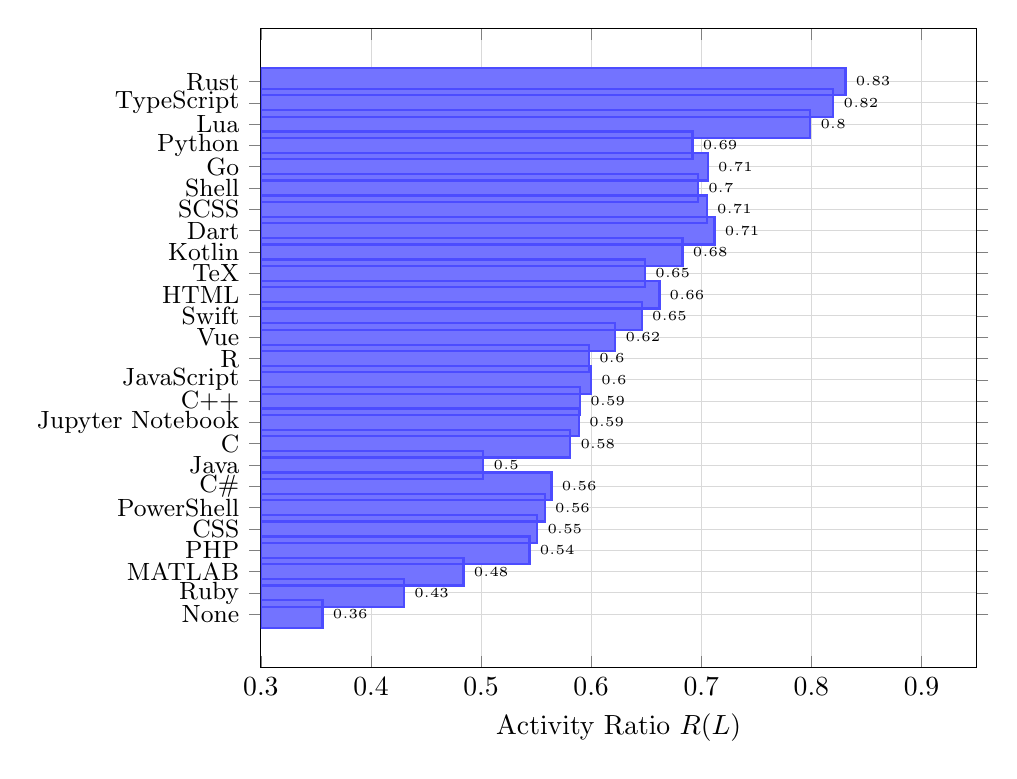
\begin{tikzpicture}
\begin{axis}[
    width=0.88\textwidth,
    height=0.80\textwidth,
    xbar,
    xmin=0.30, xmax=0.95,
    xlabel={Activity Ratio $R(L)$},
    symbolic y coords={
        None,Ruby,MATLAB,PHP,CSS,PowerShell,C\#,Java,C,
        Jupyter Notebook,C++,JavaScript,R,Vue,Swift,
        HTML,TeX,Kotlin,Dart,SCSS,Shell,Go,Python,Lua,TypeScript,Rust
    },
    ytick=data,
    yticklabel style={font=\small},
    grid=major,
    grid style={line width=0.3pt, draw=gray!30},
    every axis plot/.append style={thick},
    nodes near coords,
    nodes near coords style={font=\tiny, anchor=west},
    nodes near coords align={horizontal},
]
\addplot[fill=blue!55, draw=blue!70] coordinates {
    (0.356,None)
    (0.430,Ruby)
    (0.484,MATLAB)
    (0.544,PHP)
    (0.551,CSS)
    (0.558,PowerShell)
    (0.564,C\#)
    (0.502,Java)
    (0.581,C)
    (0.589,Jupyter Notebook)
    (0.590,C++)
    (0.600,JavaScript)
    (0.598,R)
    (0.622,Vue)
    (0.646,Swift)
    (0.662,HTML)
    (0.649,TeX)
    (0.683,Kotlin)
    (0.712,Dart)
    (0.705,SCSS)
    (0.697,Shell)
    (0.706,Go)
    (0.692,Python)
    (0.799,Lua)
    (0.820,TypeScript)
    (0.831,Rust)
};
\end{axis}
\end{tikzpicture}
\caption{Activity ratios $R(L)$ for the twenty-five largest language populations in the dataset. Languages are ordered by ratio from lowest (None, Ruby) to highest (TypeScript, Rust), revealing a temporal stratification that tracks ecosystem age and growth phase.}
\label{fig:ratios}
\end{figure}

\subsection{Median Developer Lifetimes}

Median observed lifetimes by language reveal additional structure. Languages associated with smaller or more specialized communities tend to exhibit longer lifetimes. Emacs Lisp developers show a median lifetime of $12.20$ years, followed by Elixir at $11.95$, Clojure at $11.70$, and Common Lisp at $10.73$. Vim Script developers exhibit a median of $10.40$ years, while Go and Rust developers show lifetimes of approximately $8.35$ and $8.30$ years respectively. This difference is interpretable not as reduced retention among Go and Rust developers, but rather as an artefact of limited historical depth in younger ecosystems whose developers have simply had less elapsed time to accumulate long observed lifetimes.

\subsection{Emerging Ecosystems}

Several newer ecosystems exhibit exceptionally high activity ratios: Astro at $0.90$, MDX at $0.84$, Rust at $0.83$, and TypeScript at $0.82$. These values indicate that these ecosystems are still in a growth phase, characterized by a relatively small inactive population and a high ratio of new entrants to legacy participants.

\section{Discussion}

\subsection{Developer Activity as a Survival Process}

The observed survival curve suggests that developer activity on GitHub can be modeled as a stochastic process with a characteristic decay timescale. The empirical half-life of approximately ten years indicates that participation is neither short-lived nor permanent, but instead follows a structured lifecycle.

This behavior is consistent with a hazard-based interpretation. Let $h(\tau)$ denote the hazard rate of becoming inactive at age $\tau$. The relatively smooth decline of $S(\tau)$ over the first decade suggests a moderately increasing hazard rate during early and mid-career stages, followed by stabilization among long-term participants. The increase in $S(\tau)$ for large $\tau$ is not indicative of renewed activity but rather reflects survivorship bias: developers who remain active after many years constitute a selected subset with lower effective hazard rates.

\subsection{A Generative Model of Developer Participation}

The empirical results suggest that developer activity can be modeled as a birth-death process on a population of participants. Let $N(t)$ denote the number of active developers at time $t$ within a given ecosystem, and let $n(\tau, t)$ denote the density of developers of age $\tau$ at time $t$. The evolution of the active population can be approximated by
\[
\frac{dN}{dt} = \lambda_{\text{entry}}(t) - \int_0^\infty \lambda_{\text{exit}}(\tau)\, n(\tau, t)\, d\tau,
\]
where $\lambda_{\text{entry}}(t)$ is the rate at which new developers join and $\lambda_{\text{exit}}(\tau)$ is the age-dependent rate at which active developers become inactive.

In steady-state conditions, the activity ratio $R(L)$ can be interpreted as proportional to the balance between these two processes:
\[
R(L) \;\sim\; \frac{\lambda_{\text{entry}}}{\lambda_{\text{entry}} + \lambda_{\text{exit}}}.
\]
Rapidly growing ecosystems are characterized by $\lambda_{\text{entry}} \gg \lambda_{\text{exit}}$, while declining ecosystems satisfy the opposite inequality. This model provides a mechanistic interpretation of the observed stratification of programming languages and connects the cross-sectional activity ratio to underlying population dynamics.

\subsection{Ecosystem Age and Activity Ratios}

The activity ratio $R(L)$ serves as a proxy for the temporal phase of a programming language ecosystem, reflecting the balance between entry and exit processes. Under this interpretation, high $R(L)$ indicates growing ecosystems with high entry relative to exit, intermediate $R(L)$ indicates mature and stable ecosystems, and low $R(L)$ indicates declining ecosystems with accumulated inactive users. This framework explains the observed ordering: Rust and TypeScript occupy a growth phase, Python and Go a mature phase, and Java and Ruby a declining phase relative to the snapshot captured by this dataset.

\subsection{Hazard Function Estimation}

Let $S(\tau)$ denote the empirical survival function. The corresponding discrete hazard function is approximated by
\[
h(\tau) \approx 1 - \frac{S(\tau+1)}{S(\tau)},
\]
which estimates the probability that a developer becomes inactive between age $\tau$ and $\tau+1$, conditioned on being active at age $\tau$. The gradual decline of $S(\tau)$ implies a relatively low but initially increasing hazard rate over the first decade.

A natural candidate for parametric modeling is the Weibull distribution:
\[
S(\tau) = \exp\!\left( -(\lambda \tau)^k \right),
\]
where $k > 1$ corresponds to increasing hazard. Taking logarithms yields
\[
\log(-\log S(\tau)) = k \log \tau + k \log \lambda,
\]
suggesting estimation of $k$ and $\lambda$ via linear regression on transformed data. Preliminary inspection indicates $k$ slightly greater than $1$, implying mild aging effects in developer participation. For $k = 1$ the model reduces to exponential decay with constant hazard, while $k < 1$ would indicate a decreasing hazard characteristic of strong early selection. The empirical data suggests a mixture of mildly increasing hazard and survivorship bias, resulting in the non-monotonic observed survival curve.

\subsection{Generational Structure of Programming Languages}

The results suggest that programming language ecosystems evolve in generational waves, each characterized by rapid adoption, sustained activity, and eventual saturation. A simplified periodization consistent with the data places Ruby, PHP, and early JavaScript as dominant ecosystems from roughly 2008 to 2013, with Python and modern JavaScript frameworks dominant from 2014 to 2018, and Rust, Go, and TypeScript as the leading ecosystems from 2019 to the present. As each generation matures, its activity ratio declines due to the accumulation of inactive participants. Newer ecosystems exhibit higher ratios because they have not yet accumulated such historical mass.

\subsection{Language Migration and Ecosystem Transitions}

Although this study assigns a single primary language to each developer, the observed generational structure strongly implies that developers migrate between ecosystems over time. This process can be conceptualized as a transition system on a discrete state space of languages. Let $P(L_i \to L_j)$ denote the probability that a developer transitions from language $L_i$ to language $L_j$ over a given time interval. While direct estimation of $P$ requires longitudinal data, the cross-sectional patterns observed here imply dominant transition pathways such as Ruby to JavaScript or TypeScript, Java to Kotlin, Objective-C to Swift, and JavaScript to TypeScript. These transitions reflect technological shifts and platform evolution rather than purely individual preferences.

\subsection{Niche Ecosystems and Retention}

Languages such as Emacs Lisp, Clojure, and Common Lisp exhibit unusually long median lifetimes. Such ecosystems are characterized by smaller community size, higher specialization, and stronger identity or tooling dependence. These properties may lead to lower exit rates, resulting in longer observed developer lifetimes. This suggests a trade-off between ecosystem size and retention: large ecosystems attract many participants but also experience higher turnover, while niche ecosystems retain fewer but more persistent developers.

\subsection{Entropy and Ecosystem Aging}

The accumulation of inactive accounts within a language ecosystem can be interpreted as a form of entropy increase. As ecosystems mature, they accumulate historical artifacts---repositories, accounts, and code---that no longer participate in active development. Let $I(t)$ denote the number of inactive accounts in an ecosystem. In the absence of removal processes, $dI/dt \geq 0$, leading to a monotonic dilution of the active fraction and a corresponding decline in activity ratio. New ecosystems begin with low entropy and high activity ratios, which decline as the system ages. This entropic interpretation is consistent with the observed ordering of ecosystems and provides a thermodynamic analogy for the dynamics of participation.

\subsection{Network Effects and Visibility Bias}

The use of a follow network introduces a structural bias toward developers who are socially visible. This inflates the observed activity rate and amplifies the representation of ecosystems associated with infrastructure, tooling, and open source leadership. More formally, let $w_i$ denote the probability that developer $i$ is included in the sample. Then
\[
w_i \propto f(F_i, A_i),
\]
where $F_i$ is follower count, $A_i$ is activity, and $f$ is an increasing function of both quantities. The observed estimator of the survival function accordingly overestimates the true survival probability. Correcting for this bias would require reweighting observations or incorporating independent sampling strategies.

\subsection{Activity as Constraint Satisfaction}

An alternative interpretation of developer activity frames continued participation as a form of ongoing constraint satisfaction. Developers remain active as long as they can maintain alignment between personal interest, available time, economic incentives, and ecosystem relevance. In this view, inactivity arises not from a single cause but from the gradual accumulation of constraint violations. This perspective is consistent with the observed gradual decay of activity rather than abrupt transitions and connects the empirical survival curve to an underlying process of resource and motivation dynamics.

\subsection{The Role of Non-Code Accounts}

The large \texttt{None} category plays a central role in the structure of inactivity. Its low activity ratio of $0.356$ indicates that accounts without active repository engagement are substantially more likely to become inactive. This suggests that participation in code production---rather than mere presence on the platform---is a key determinant of long-term engagement. The disproportionate representation of this group among inactive accounts ($39.68\%$ of all inactive accounts) implies that any aggregate estimate of platform-wide activity rates depends critically on how this population is treated.

\section{Limitations}

\subsection{Sampling Bias}

The dataset is derived from a follow network and is therefore not a uniform sample of GitHub users. It is likely biased toward developers who are socially visible, connected, or of particular interest to the source account. This bias inflates the observed activity rate and may overrepresent certain ecosystems.

\subsection{Activity Proxy}

Activity is defined based on public repository pushes within a one-year window. This measure does not capture private repository activity, non-code contributions such as issues and reviews, or activity conducted outside the GitHub platform. Some developers classified as inactive may therefore remain active in other contexts not reflected in the data.

\subsection{Language Attribution}

Assigning a single language based on the most recent repository is a simplification. Many developers work across multiple languages, and the chosen proxy reflects only their most recent visible activity. Developers working primarily in private or multi-language contexts may be systematically misclassified.

\subsection{Right-Censoring}

Observed lifetimes are right-censored for active users. As a result, median lifetime estimates are conservative and may substantially underestimate true participation durations. A more accurate estimator would require Kaplan--Meier methods or equivalent longitudinal tracking.

\section{Toward a Unified Model of Developer Ecosystems}

The results suggest that developer ecosystems can be understood as dynamical systems characterized by interacting entry and exit processes, temporal survival dynamics, migration between language states, and monotonic accumulation of inactive mass. These components can be integrated into a unified model in which programming languages are viewed not merely as tools but as evolving attractors in a high-dimensional space of developer behavior. Under this model, the activity ratio of a language serves as an order parameter encoding its current position in a lifecycle from emergence through maturity to decline. Such a model would enable prediction of ecosystem growth, decline, and transition, and would provide a quantitative framework for understanding the evolution of software development at scale.

\section{Conclusion}

This study provides a large-scale, developer-centered analysis of activity on GitHub using a dataset of over $370{,}000$ accounts. Developer activity follows a structured lifecycle with a characteristic half-life of approximately ten years. Programming language ecosystems exhibit systematic variation in activity ratios, reflecting their stage of evolution: newer ecosystems show high activity due to growth, while older ecosystems accumulate inactive participants over time. A substantial fraction of inactive accounts are associated with no identifiable primary language, indicating limited or absent repository activity and identifying repository engagement as a key determinant of long-term participation.

These findings suggest that both individual participation and ecosystem dynamics can be understood within a unified temporal framework. GitHub, viewed at scale, is not a static repository of code but a dynamic system shaped by generational turnover and evolving technological landscapes. Future work may extend this analysis by incorporating longitudinal data, modeling transitions between ecosystems, applying Kaplan--Meier estimation to account for right-censoring, and integrating additional signals such as collaboration networks and contribution types.

\bibliographystyle{plainnat}

\begin{thebibliography}{9}

\bibitem[Kalliamvakou et al.(2014)]{kalliamvakou2014promises}
Eirini Kalliamvakou et al.
\newblock The promises and perils of mining GitHub.
\newblock In \emph{MSR}, 2014.

\bibitem[Gousios(2014)]{gousios2014ghtorrent}
Georgios Gousios.
\newblock The GHTorrent dataset and tool suite.
\newblock In \emph{MSR}, 2014.

\bibitem[Zhou and Mockus(2016)]{zhou2016information}
Minghui Zhou and Audris Mockus.
\newblock Who will stay in the FLOSS community?
\newblock \emph{IEEE Transactions on Software Engineering}, 2016.

\bibitem[Vasilescu et al.(2015)]{vasilescu2015gender}
Bogdan Vasilescu et al.
\newblock Gender and tenure diversity in GitHub teams.
\newblock In \emph{CHI}, 2015.

\bibitem[Joblin et al.(2017)]{joblin2017classifying}
Mitchell Joblin et al.
\newblock Classifying developers into core and peripheral roles.
\newblock In \emph{ICSE}, 2017.

\end{thebibliography}

\appendix

\section{Mathematical Appendix}

\subsection{Discrete Survival Estimation}

Let $\tau \in \mathbb{N}$ denote account age in years. For each age bin $\tau$, define
\[
N(\tau) = N_{\text{active}}(\tau) + N_{\text{inactive}}(\tau),
\qquad
S(\tau) = \frac{N_{\text{active}}(\tau)}{N(\tau)}.
\]
This defines a discrete cross-sectional estimate of the survival function $S(\tau) \approx P(\text{active} \mid \text{age} = \tau)$. Unlike classical longitudinal survival analysis, this estimator assumes that the distribution of account ages approximates a stationary population.

\subsection{Discrete Hazard Function}

The discrete hazard function is approximated by
\[
h(\tau) \approx 1 - \frac{S(\tau+1)}{S(\tau)} = \frac{S(\tau) - S(\tau+1)}{S(\tau)},
\]
which estimates the probability that a developer becomes inactive between age $\tau$ and $\tau+1$, conditioned on being active at age $\tau$. The gradual decline of $S(\tau)$ implies a relatively low but increasing hazard rate over the first decade.

\subsection{Half-Life Estimation}

The activity half-life $\tau_{1/2}$ is defined implicitly by $S(\tau_{1/2}) = 1/2$. Given discrete observations, we estimate
\[
\tau_{1/2} \approx \min\{\tau : S(\tau) \leq 0.5\},
\]
which in the present dataset occurs near $\tau \approx 10$ years.

\subsection{Right-Censoring}

For active accounts, the true lifetime $\ell^*$ satisfies $\ell^* \geq \ell = t_{\text{push}} - t_{\text{create}}$. Observed lifetimes are therefore right-censored, and the median lifetime computed from observed $\ell$ underestimates the true median. A more accurate estimator would apply the Kaplan--Meier procedure:
\[
\hat{S}(\tau) = \prod_{\tau_i \leq \tau} \left(1 - \frac{d_i}{n_i}\right),
\]
where $d_i$ is the number of exits at time $\tau_i$ and $n_i$ is the number at risk.

\subsection{Activity Ratio as a Mixture Statistic}

Let $T$ denote the random variable representing developer lifetime. Then
\[
R(L) \approx P(T > \Delta \mid L),
\]
where $\Delta = 1$ year is the activity cutoff. Thus $R(L)$ estimates the survival probability beyond a fixed horizon, making it a special case of the survival function evaluated at a single time point.

\subsection{Bias from Cross-Sectional Sampling}

The estimator $S(\tau)$ is biased by the age distribution of accounts. Let $\pi(\tau)$ denote the probability of sampling an account of age $\tau$. The observed survival function is
\[
S_{\text{obs}}(\tau) = P(\text{active} \mid \tau, \text{sampled}),
\]
which depends on $\pi(\tau)$. If older accounts are overrepresented, the survival curve may be biased upward at large $\tau$. Combined with the visibility weighting described below, this produces upward bias both at large $\tau$ and in aggregate activity estimates.

\subsection{Visibility-Weighted Sampling}

Let $w_i$ denote the inclusion probability of account $i$ in the follow network, with $w_i \propto f(F_i, A_i)$ where $F_i$ is follower count and $A_i$ is activity level. The observed survival estimator becomes
\[
S_{\text{obs}}(\tau) = \frac{\sum_i w_i \,\mathbf{1}_{\{\text{active},\, \tau_i = \tau\}}}{\sum_i w_i \,\mathbf{1}_{\{\tau_i = \tau\}}}.
\]
Since $w_i$ increases with activity, $S_{\text{obs}}(\tau)$ overestimates the true survival probability. Correcting for this bias requires either Horvitz--Thompson reweighting or an independent sampling frame.

\subsection{Confidence Intervals}

For each age bin, the standard error of $S(\tau)$ is approximated by
\[
\mathrm{SE}(\tau) = \sqrt{\frac{S(\tau)(1 - S(\tau))}{N(\tau)}}.
\]
A $95\%$ confidence interval is $S(\tau) \pm 1.96 \cdot \mathrm{SE}(\tau)$. Given the large sample sizes in this dataset, these intervals are narrow, implying high statistical confidence in aggregate estimates.

\subsection{Weibull Model Fit}

The Weibull survival model $S(\tau) = \exp(-(\lambda \tau)^k)$ yields, upon logarithmic transformation,
\[
\log(-\log S(\tau)) = k \log \tau + k \log \lambda,
\]
enabling estimation of $k$ and $\lambda$ by linear regression on the log-log scale. When $k > 1$ the hazard is increasing (aging effect); when $k = 1$ the hazard is constant (memoryless exponential); when $k < 1$ the hazard is decreasing (early selection). The empirical data suggests $k$ slightly greater than $1$, indicating a mild aging effect consistent with gradual disengagement over the developer lifecycle.

\subsection{Limit of Large Time}

As $\tau \to \infty$, the observed survival function approaches
\[
\lim_{\tau \to \infty} S(\tau) = P(\text{persistent developer}),
\]
which represents the long-run fraction of the population composed of highly persistent users. The upward trend in $S(\tau)$ at large $\tau$ is therefore interpretable as convergence to this limiting value under a mixture model in which the population contains a subpopulation of developers with effectively zero exit hazard.

\end{document}
